\documentclass[12pt]{article}

\usepackage{amsmath}
\usepackage{latexsym}
\usepackage{amstext}
\usepackage{array}
\usepackage{multirow}
\usepackage{graphicx}
\usepackage{caption}
\usepackage{subcaption}
\title{Creating looped Polymer by Brownian Bridges- implications for polymer dynamics simulations}
\begin{document}
\maketitle
Given a linear polymer of $N$ beads, and a set of pairs of bead indices to connect into loops, we use the Brownian bridge transformation on the linear polymer to iteratively loop it accordingly. Since a random initial configuration of the Gaussian chain does not differ by its random configuration after relaxation time, we can save simulation time by starting with a looped polymer. 

First, some terms. The indices of a begining and end of loop form an interval on the linear polymer. This interval can either contain or be contained by other intervals, contain the start/end index of another interval, or not contain any other interval. 

The procedure goes as follows 
\begin{enumerate}
\item classify the loops to those containing other loops and those who don't.\\
\begin{figure}[H!]
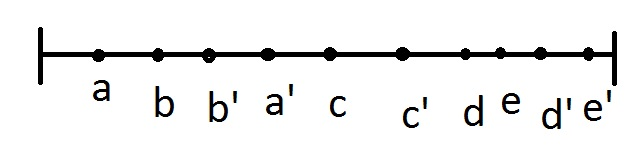
\includegraphics[scale=0.2]{possibleIntervalArrangements}
\caption{four types of intervals. [a a'] contains [b b'], [c c'] is not contained, [d d'] contains the start of [e e']}
\label{figure_possibleIntervalArrangements}
\end{figure}
\item
\end{enumerate}

 
\end{document}